% From https://texample.net/tikz/examples/three-link-manipulator/

\documentclass{article}

\usepackage{tikz}
\usetikzlibrary{patterns}
\usetikzlibrary{positioning,fit}
\usetikzlibrary{decorations.markings}


\begin{document}
\pagestyle{empty}

% Define a variable as a length
\newcommand{\nvar}[2]{%
    \newlength{#1}
    \setlength{#1}{#2}
}

% Define a few constants for drawing
\nvar{\dg}{0.3cm}
\def\dw{0.25}\def\dh{0.5}
% Define commands for links, joints and such
\def\link{\draw [double distance=1.5mm, very thick] (0,0)--}
\def\joint{%
    \filldraw [fill=white] (0,0) circle (5pt);
    \fill[black] circle (2pt);
}
\def\grip{%
    \draw[ultra thick](0cm,\dg)--(0cm,-\dg);
    \fill (0cm, 0.5\dg)+(0cm,1.5pt) -- +(0.6\dg,0cm) -- +(0pt,-1.5pt);
    \fill (0cm, -0.5\dg)+(0cm,1.5pt) -- +(0.6\dg,0cm) -- +(0pt,-1.5pt);
}

\def\robotbase{%
    \draw[rounded corners=8pt] (-\dw,-\dh)-- (-\dw, 0) --
    (0,\dh)--(\dw,0)--(\dw,-\dh);
    \draw (-0.5,-\dh)-- (0.5,-\dh);
    \fill[pattern=north east lines] (-0.5,-1) rectangle (0.5,-\dh);
}

% This macro draws a three link manipulator.
% Input parameters:
%   #1 theta_1
%   #2 L_1
%   #3 theta_2
%   #4 L_2
%   #5 theta_3
%   #6 L_3
%
% Example:
%   \threelink{60}{2}{-70}{2}{30}{1}
\newcommand{\threelink}[6]{%
    \robotbase
    \link(#1:#2);
    \joint
    \begin{scope}[shift=(#1:#2), rotate=#1]
        \link(#3:#4);
        \joint
        \begin{scope}[shift=(#3:#4), rotate=#3]
            \link(#5:#6);
            \joint
            \begin{scope}[shift=(#5:#6), rotate=#5]
                \grip
            \end{scope}
        \end{scope}
    \end{scope}
}

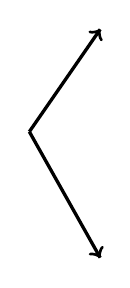
\begin{tikzpicture}
    \begin{scope}
        \threelink{70}{2}{-130}{2}{60}{1}
    \end{scope}

    \begin{scope}[xshift=4cm,yshift=2cm,scale=0.5, every node/.append style={transform shape}]
        \threelink{60}{2}{-110}{2}{90}{1}
    \end{scope}

    \begin{scope}[xshift=4cm,yshift=-2cm,scale=0.5, every node/.append style={transform shape}]
        \threelink{60}{2}{-110}{2}{30}{1}
    \end{scope}

    % draw arrows between the scopes above
    \begin{scope}[very thick,decoration={
                    markings,
                    mark=at position 1.0 with {\arrow{>}}}
        ]
        \draw[postaction={decorate}] (3,0.15)--(3.9,1.45);
        \draw[postaction={decorate}] (3,0.15)--(3.9,-1.45);
    \end{scope}


\end{tikzpicture}

\end{document}
